\subsection{Versuchsaufbau}\label{subsec:Versuchsaufbau}
Für den Versuchsaufbau wurde der BLDC mit einer Asynchronmaschine (ASM) gekoppelt, welche über einen Frequenzumrichter angesteuert wird und netzspeisefähig ist. Die ASM simuliert bei den nachfolgenden Versuchen die Last.


\begin{figure}[H]
	\begin{center}
		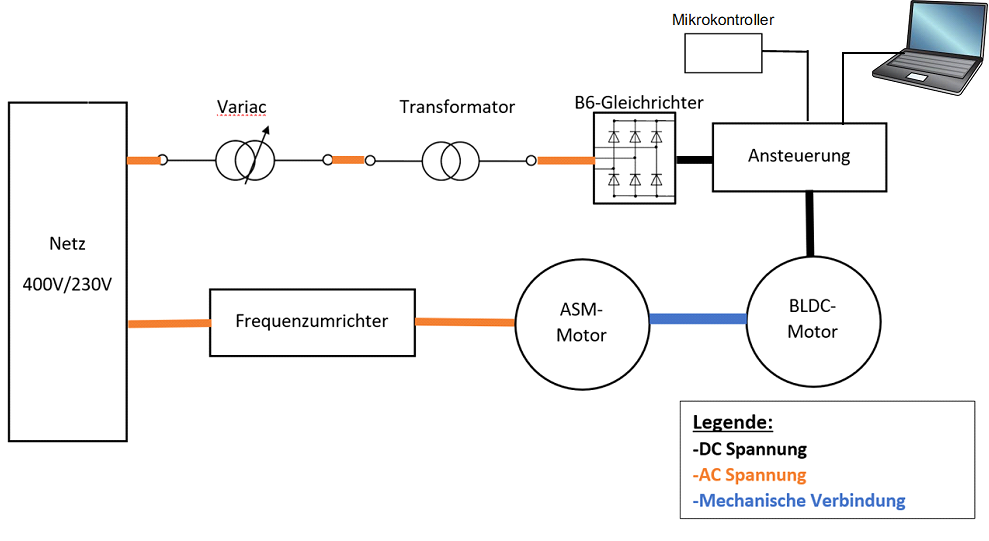
\includegraphics[height=70mm]{Versuchsaufbau/Schema3.png}
		\caption{Schema Versuchsaufbau}
		\label{fig:Schema}
	\end{center}
\end{figure}

Folgende Messgrössen sind in den Versuchen gemessen worden:
\begin{itemize}
	\item Die \textbf{Spannung} im Zwischenstromkreis, zwischen B6-Gleichrichter und Ansteuerung, wurde mit einem digitalen Multimeter gemessen.
	\item Der \textbf{Strom} im Zwischenstromkreis, zwischen B6-Gleichrichter und Ansteuerung, wurde mithilfe einer Strommesszange und einem Oszilloskop gemessen.
	\item Die \textbf{Drehzahl} wurde mit einem Oszilloskop gemessen, welches den Hallsensor des BLDC-Motors ausgewertet hat. Da der Motor vier Pole hat, generiert dieser vier Impulse pro Umdrehung.
	\item Die \textbf{Leistung} wurde mit einem Power-Analyzer zwischen der ASM und dem Frequenzumrichter gemessen.
	\item Der \textbf{Drehmoment-Sollwert} wurde digital mit einem Mikrocontroller erzeugt und auf die Ansteuerung gegeben.
	\item Die \textbf{Motor-Temperatur} konnte mit dem Computer und der mitgelieferten Software ausgelesen werden. Der Computer war via USB-Verbindung mit der Ansteuerung verbunden.
	\item Die \textbf{Controller-Temperatur} wurde ebenfalls mit dem Computer und der mitgelieferten Software ausgewertet.
\end{itemize}

Wie auf dem Schema in Abbildung \ref{fig:Schema} ersichtlich, erfolgt die Stromversorgung des BLDC Motors über Variac, Transformatoren und Gleichrichter. Dieser \glqq komplizierte \grqq Aufbau war notwendig, da keine Stromquelle gefunden werden konnte, welche genügend Leistung (im Vergleich zur Nennleistung des BLDC) brachte. Da der Brushless-DC-Motor für den Betrieb eine konstante Spannung von 96V und unter Volllast ($\approx$15kW) Ströme bis über 160A benötigt, musste ein Aufbau wie im Schema ersichtlich gewählt werden. Dabei erfolgt die Energieversorgung durch das 400V-Drehstromnetz. Mithilfe des Variacs, welcher mit einer CEE-63A-Steckdose am Netz angeschlossen war, liess sich die Spannung im Zwischenstromkreis regeln. Der Variac ist für eine Ausgangsspannung zwischen 0-290V und einen maximalen Strom von 50A ausgelegt. Damit der BLDC-Motor seine Betriebsspannung von lediglich 96V und Ströme von deutlich über 100A erhält, wurde ein Transformator mit einem 1:3 Übersetzungsverhältnis nachgeschaltet. Dadurch konnte eine dreimal höhere Spannung am Variac eingestellt werden, wodurch sich der Strom um denselben Faktor verringert. Der Anschluss des Transformator erfolgte primärseitig und sekundärseitig in Dreieckschaltung und hat einen sekundären Maximalstrom von $95A_{AC}$ bei $127V_{AC}$. Die Gleichrichtung erfolgt mit einer B6-Brücke, welche für das Projekt aufgebaut wurde. Der Aufbau ist in Abbildung \ref{fig:B6} ersichtlich.

\begin{figure}[H]
	\centering
	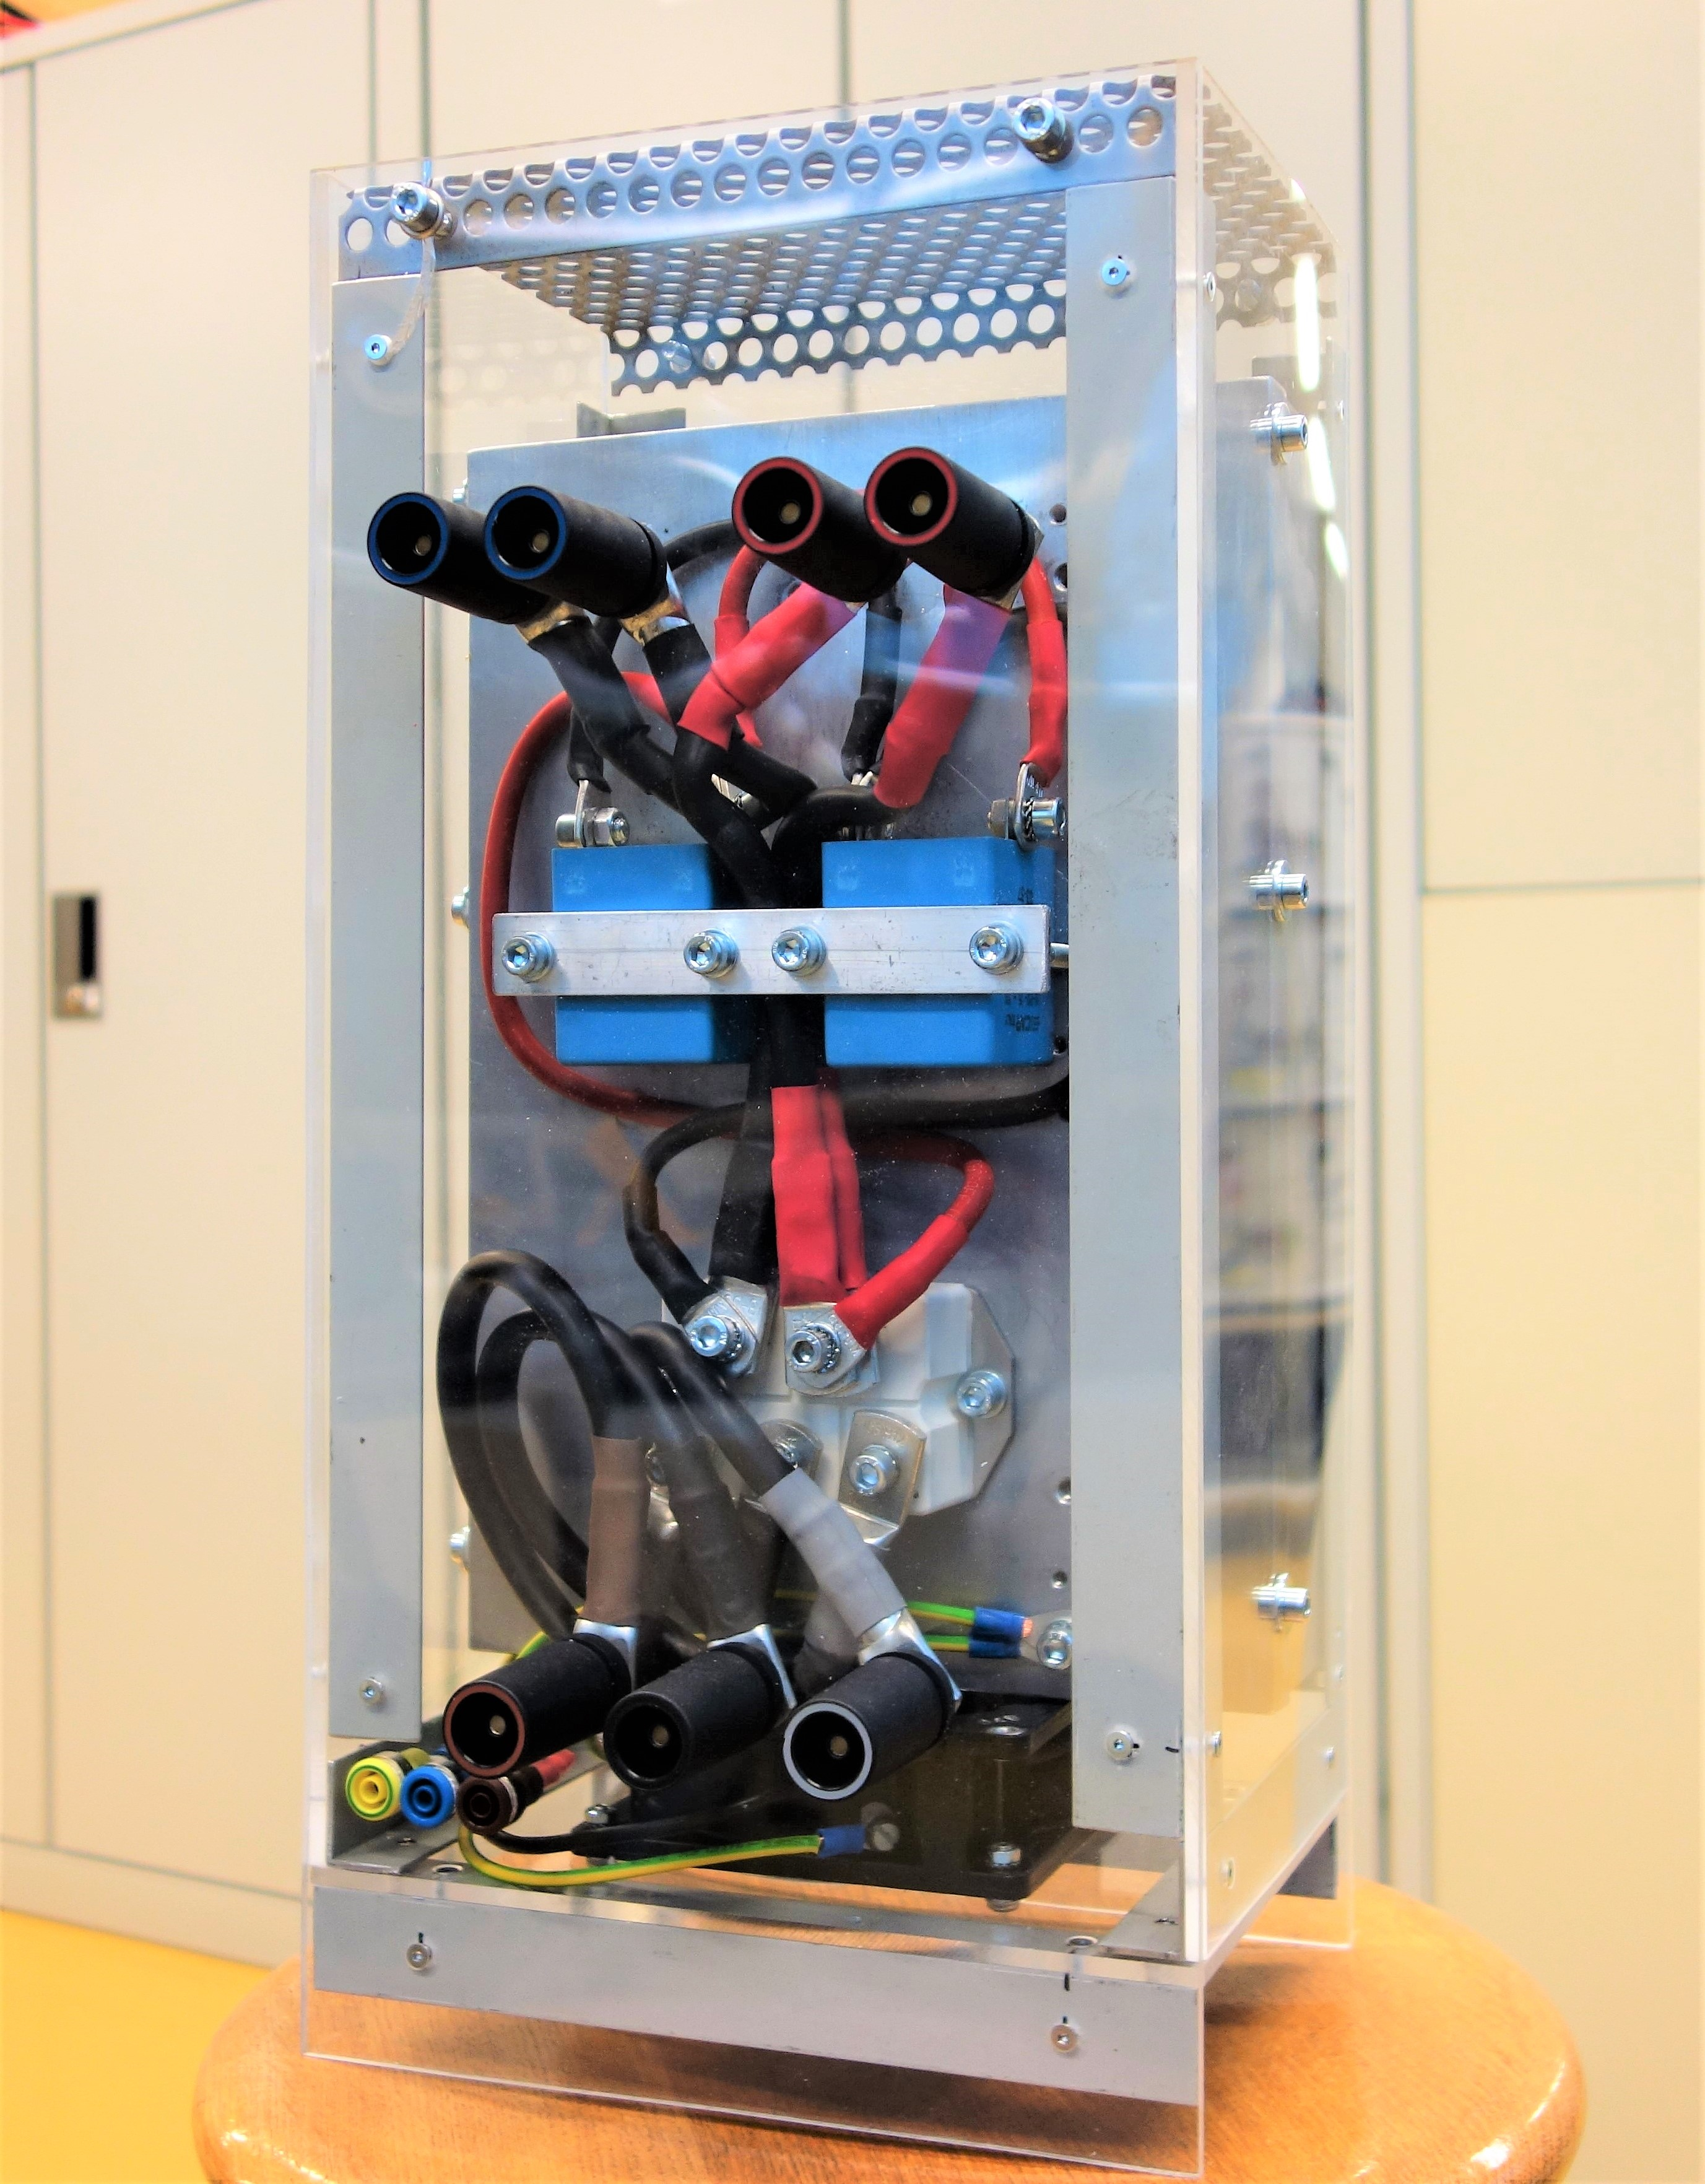
\includegraphics[width=60mm]{Versuchsaufbau/DSC00547(2).jpg}
	\caption[B6-Gleichrichter]{B6-Gleichrichter}
	\label{fig:B6}
\end{figure}

Die AC-Einspeisung der B6-Brücke erfolgt durch die drei Klemmen (braun, schwarz, grau) im unteren Bereich. Diese werden auf den eigentlichen Diodengleichrichter (weiss) und zwei Stützkondensatoren (blau) geführt. Alle Bauteile des B6-Gleichrichter wurden auf einen Nennstrom von 200A im Zwischenstromkreis (DC-Seite) ausgelegt. Da die Stecker nicht für einen solch hohen Strom ausgelegt sind, wurden die Verbindungen auf der DC-Seite doppelt geführt. Das Stromverhältnis zwischen dem Zwischenstromkreis und dem Leiterstrom auf der AC-Seite, lässt sich mit nachfolgender Formel \ref{eq:B6-Strom} berechnen.

\begin{equation}
\centering
I_{d}=\frac{I_{A,rms}}{\sqrt{\frac{2}{3}}}
\label{eq:B6-Strom}
\end{equation}
$ I_{d} $\qquad\quad 	Zwischenkreisstrom (DC-Seite)      \\
$ I_{A,rms} $\quad Leiterstrom (AC-Seite)    \\

Werden alle Stromgrenzen betrachtet, dann wird ersichtlich, dass der Versuchsaufbau durch die Strombelastbarkeit des Transformators begrenzt ist. Wenn der Transformator bei Volllast betrieben wird ($95A_{AC}$), dann ergibt sich dadurch beim Variac (3:1-Verhältnis) ein Strom von $33A$ und im Zwischenstromkreis (Formel \ref{eq:B6-Strom}) einen Strom von 116A.\\
Wird die Nennspannung des Motors ($96V_{DC}$) im Zwischenstromkreis eingestellt, ergibt sich auf der AC-Seite des B6-Gleichrichters eine Spannung von $71V_{AC}$ (Formel \ref{eq:B6-Spannung}) und eine Ausgangsspannung des Variacs (1:3-Verhältnis) von $213V_{AC}$.

\begin{equation}
\centering
U_{di0}=\frac{3}{\pi}\sqrt{2}\cdot U_{AD}\approx 1.35U_{AD}
\label{eq:B6-Spannung}
\end{equation}
$  U_{di0} $\quad  Zwischenkreisspannung (DC-Seite)      \\
$ U_{AD} $\quad  Verkettete Spannung (AC-Seite)        \\

Die maximale Leistung, welche mit diesem Versuchsaufbau getestet werden kann, beträgt demnach ca. 11kW (Formel \ref{eq:PUI}). Da die Versuchsdauer relativ kurz ist und die Leistung durch den Transformator begrenzt ist, welcher auf Dauerbelastung ausgelegt ist, kann der Versuchsaufbau kurzzeitig überbelastet werden. Wie im Kapitel \ref{subsec:MotorController} erläutert, ist dies auch von Nöten.

\begin{equation}
\centering
P=U_{di0}\cdot I_{d}
\label{eq:PUI}
\end{equation}
$  U_{di0} $\quad  Zwischenkreisspannung (DC-Seite)      \\
$ I_{d} $\quad\quad 	Zwischenkreisstrom (DC-Seite)      \\


Da der B6-Gleichrichter bei hoher Belastung einen grossen Stromrippel generieren, sind parallel zur Ansteuerung zwei Elektrolytkondensatoren (Elkos) eingebaut. Diese dienen zur Glättung der Gleichstromversorgung bei hohen Belastungen. Zusätzlich wurde im Zwischenstromkreis ein DC-Relais eingebaut, welches von der Ansteuerung selbst geschaltet werden kann. Tritt ein Fehlerfall auf, kann der Controller mithilfe des DC-Relais die Stromversorgung unterbrechen. Die Ansteuerung besitzt zudem eine Schmelzsicherung direkt nach der Einspeisung des +Pols.\\

Der Drehmoment-Sollwert für die Ansteuerung wird mit einem Arduino-Controller erzeugt. Dabei wird der PWM-Ausgang mithilfe eines RC-Tiefpasses in ein Spannungssignal gewandelt. Zudem wird das Signal des Hallsensors über ein Schmitt-Trigger auf den Mikrocontroller geführt, damit die Geschwindigkeit geregelt werden kann.\\
Der ASM-Motor, welcher die Last simulierte, hat ebenfalls eine Leistung von 11kW und ist starr mittels einer Kupplung mit dem BLDC-Motor gekopplet. Die Anordnung ist in Abbildung \ref{fig:Motorenaufbau} dargestellt. Damit diese zwei Maschinen überhaupt miteinander gekoppelt werden konnten, ist zuerst die Welle des BLDC-Motors (links) auf das Niveau der ASM (rechts) angehoben worden. Weiter waren einige Anpassungen an der Kupplung (Verbindung zwischen den Motorenwellen) getätigt werden. Da der BLDC-Motor über eine Welle mit Zollmass verfügt, musste die Öffnung einer Kupplung ausgebohrt worden. Weiter verfügt die ASM über keine Nut, weshalb die Befestigung der Kupplung mit zwei M8-Schrauben, welche auf die Motorwelle drücken, erfolgt. Diese zwei Gewinde sind ebenfalls vorgängig gebohrt werden. Für einen ausreichenden Berührungsschutz sorgt eine Plexiglasscheibe über der mechanischen Verbindung.

\begin{figure}[H]
	\centering
	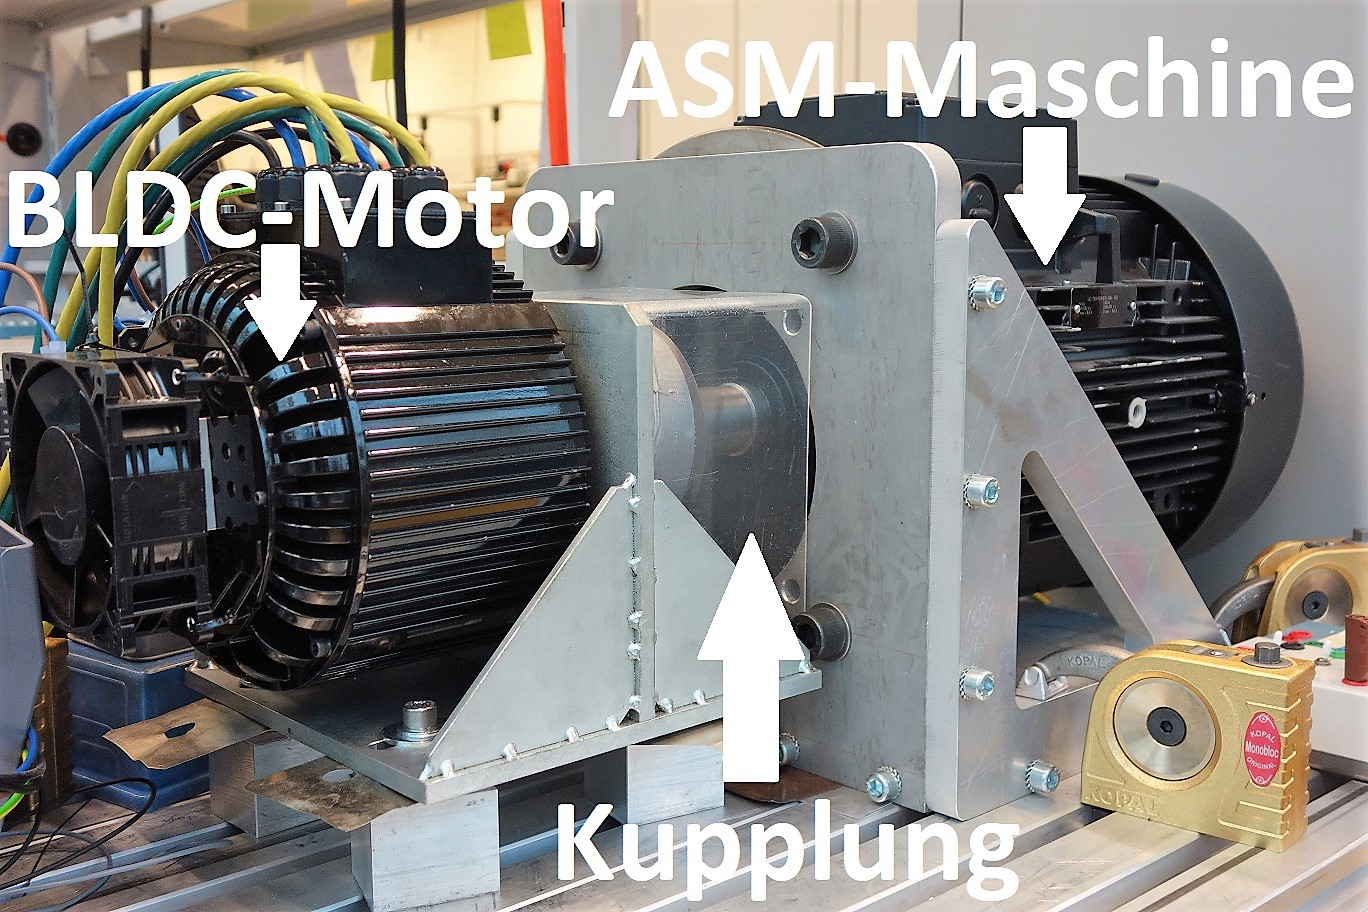
\includegraphics[width=100mm]{Versuchsaufbau/Motorenaufbau.jpg}
	\caption{Koppung des BLDC-Motors mit der ASM-Maschine}
	\label{fig:Motorenaufbau}
\end{figure}

Leider verfügt der für die Winde gekaufte Motor nur über eine schlechte Eigenkühlung, wodurch zusätzliche Ventilatoren notwendig sind. Bei den Temperaturtests \ref{subsec:Temperatur} sind zur Kühlung externe 110mm Ventilatoren verwendet worden. In Abbildung \ref{fig:Motorenlueftung}, ist die Anordnung seitlich und hinter dem Motor zu sehen.



\begin{figure}[H]
	\centering
	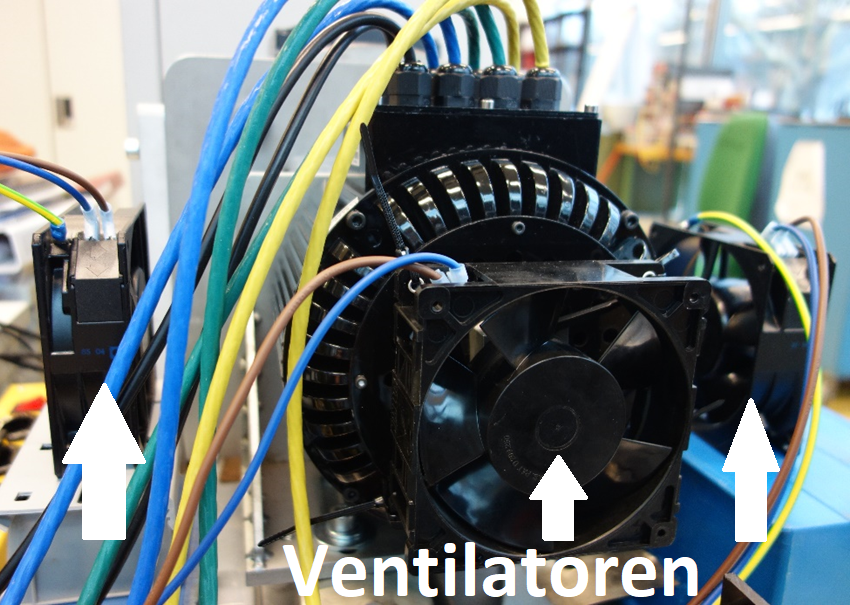
\includegraphics[width=100mm]{Versuchsaufbau/Motorenlueftung.png}
	\caption{BLDC-Motor mit zusätzlicher Lüftung}
	\label{fig:Motorenlueftung}
\end{figure}

%\begin{figure}[H]
%	\begin{center}
%		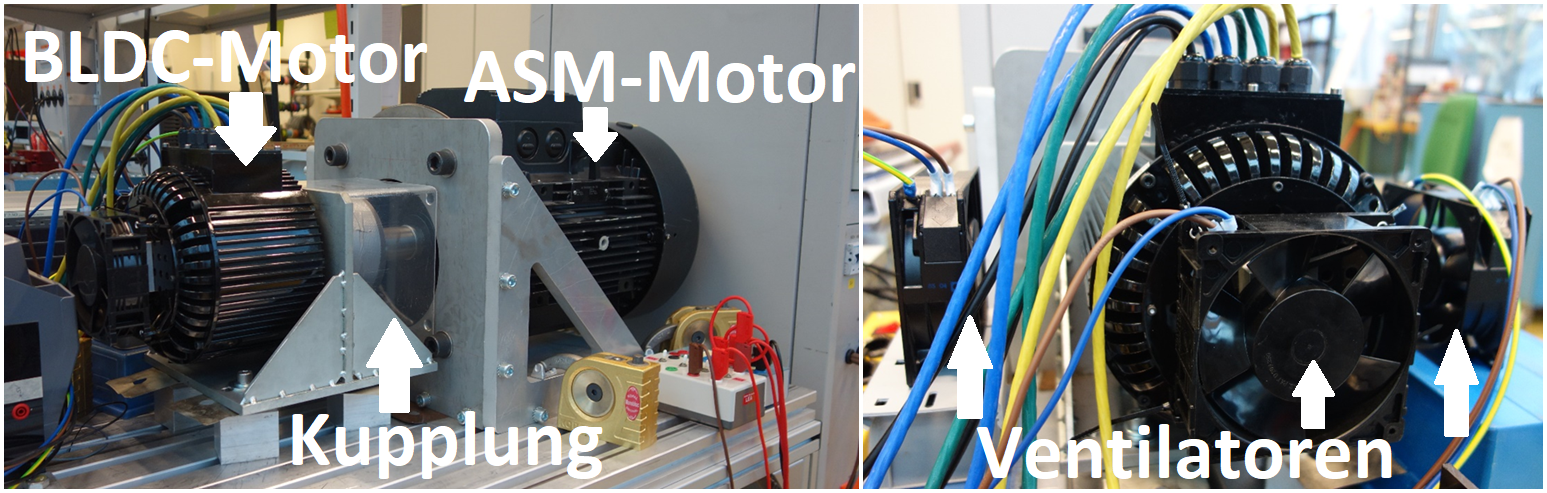
\includegraphics[width=\linewidth]{Versuchsaufbau/MotorLueft_neu.png}
%		\caption[Motoren Aufbau und Motorenlüftung]{Motoren Aufbau (links) und Motorenlüftung (rechts)}
%		\label{fig:MotorenLueftung}
%	\end{center}
%\end{figure}

Damit überhaupt Leistungsversuche möglich sind, muss neben dem Gleichstrommotor auch die ASM angesteuert werden. Hierfür dient ein Frequenzumrichter mit integrierter Netzschaltung welche ebenfalls ans 400V-Stromnetz angeschlossen ist. Während der BLDC-Motor eine Drehmoment-Ansteuerung verfügt wurde der ASM-Motor über die Drehzahl geregelt, welche wiederum von der Frequenz abhängig ist. Die Frequenz der ASM lässt sich über ein Potentiometer regeln.